\documentclass[14pt]{extbook}
\usepackage{multicol, enumerate, enumitem, hyperref, color, soul, setspace, parskip, fancyhdr} %General Packages
\usepackage{amssymb, amsthm, amsmath, latexsym, units, mathtools} %Math Packages
\everymath{\displaystyle} %All math in Display Style
% Packages with additional options
\usepackage[headsep=0.5cm,headheight=12pt, left=1 in,right= 1 in,top= 1 in,bottom= 1 in]{geometry}
\usepackage[usenames,dvipsnames]{xcolor}
\usepackage{dashrule}  % Package to use the command below to create lines between items
\newcommand{\litem}[1]{\item#1\hspace*{-1cm}\rule{\textwidth}{0.4pt}}
\pagestyle{fancy}
\lhead{Progress Quiz 6}
\chead{}
\rhead{Version C}
\lfoot{9689-6866}
\cfoot{}
\rfoot{Spring 2021}
\begin{document}

\begin{enumerate}
\litem{
Choose the equation of the function graphed below.
\begin{center}
    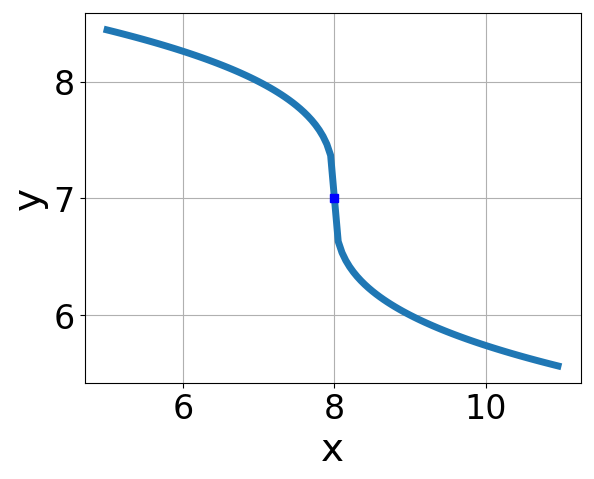
\includegraphics[width=0.5\textwidth]{../Figures/radicalGraphToEquationC.png}
\end{center}
\begin{enumerate}[label=\Alph*.]
\item \( f(x) = \sqrt{x + 14} + 4 \)
\item \( f(x) = - \sqrt{x + 14} + 4 \)
\item \( f(x) = \sqrt{x - 14} + 4 \)
\item \( f(x) = - \sqrt{x - 14} + 4 \)
\item \( \text{None of the above} \)

\end{enumerate} }
\litem{
Choose the graph of the equation below.\[ f(x) = - \sqrt{x + 14} - 3 \]\begin{enumerate}[label=\Alph*.]
\begin{multicols}{2}\item 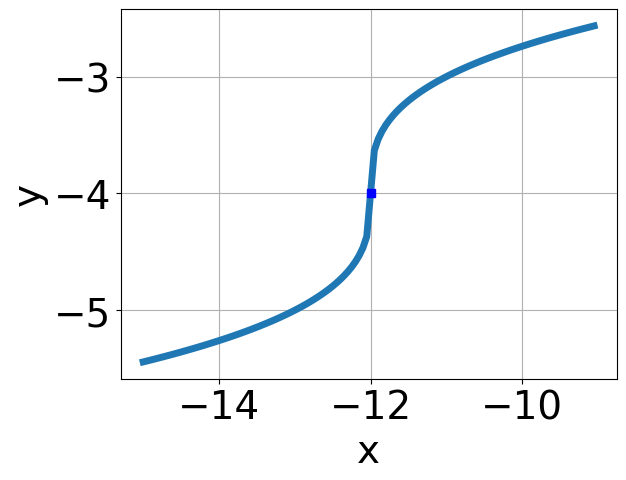
\includegraphics[width = 0.3\textwidth]{../Figures/radicalEquationToGraphCopyAC.png}\item 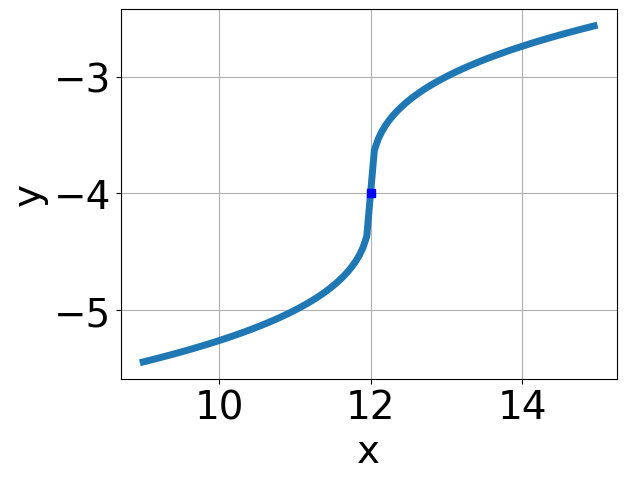
\includegraphics[width = 0.3\textwidth]{../Figures/radicalEquationToGraphCopyBC.png}\item 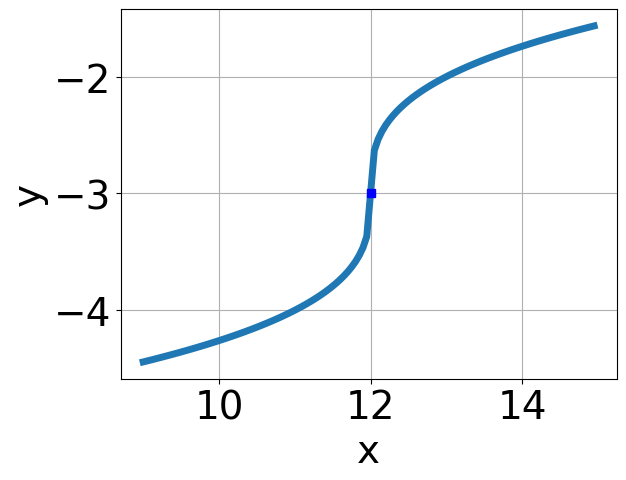
\includegraphics[width = 0.3\textwidth]{../Figures/radicalEquationToGraphCopyCC.png}\item 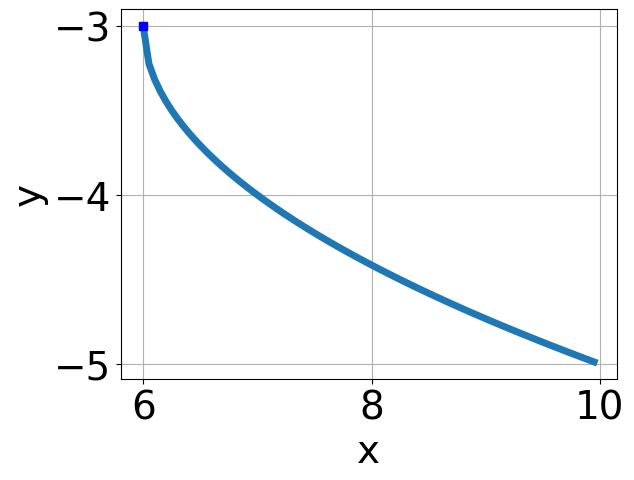
\includegraphics[width = 0.3\textwidth]{../Figures/radicalEquationToGraphCopyDC.png}\end{multicols}\item None of the above.
\end{enumerate} }
\litem{
Choose the graph of the equation below.\[ f(x) = - \sqrt{x + 10} - 7 \]\begin{enumerate}[label=\Alph*.]
\begin{multicols}{2}\item 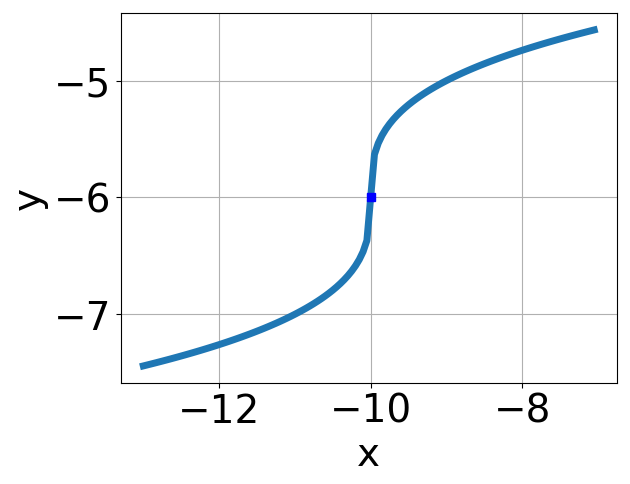
\includegraphics[width = 0.3\textwidth]{../Figures/radicalEquationToGraphAC.png}\item 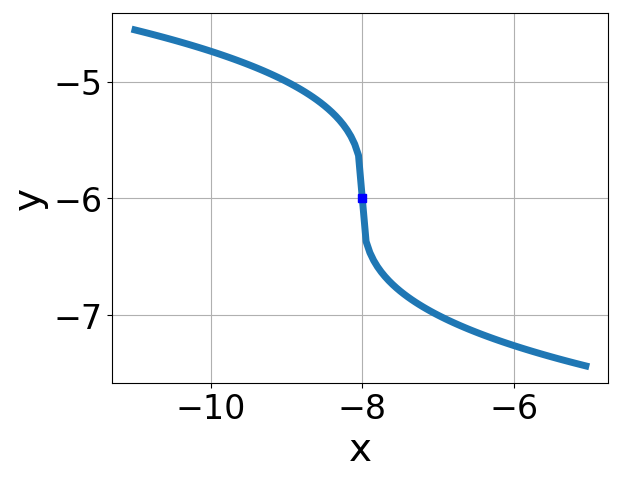
\includegraphics[width = 0.3\textwidth]{../Figures/radicalEquationToGraphBC.png}\item 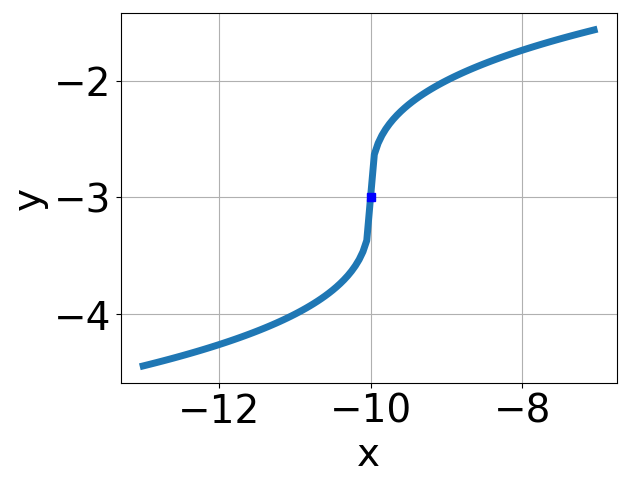
\includegraphics[width = 0.3\textwidth]{../Figures/radicalEquationToGraphCC.png}\item 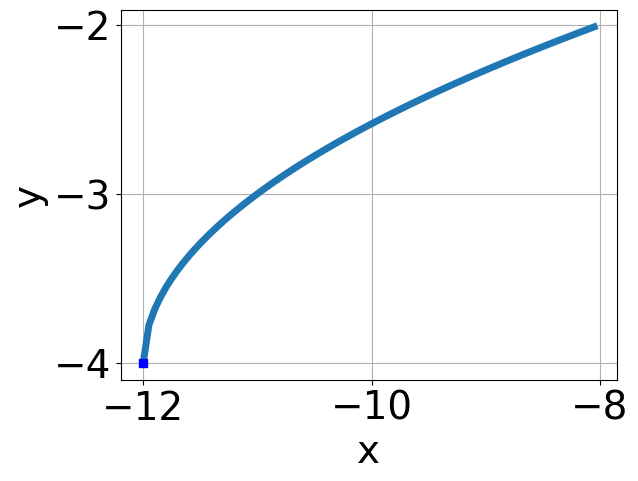
\includegraphics[width = 0.3\textwidth]{../Figures/radicalEquationToGraphDC.png}\end{multicols}\item None of the above.
\end{enumerate} }
\litem{
What is the domain of the function below?\[ f(x) = \sqrt[6]{4 x + 8} \]\begin{enumerate}[label=\Alph*.]
\item \( (-\infty, \infty) \)
\item \( [a, \infty), \text{where } a \in [-0.93, 0.16] \)
\item \( (-\infty, a], \text{where } a \in [-1.39, 1.52] \)
\item \( (-\infty, a], \text{where } a \in [-2.94, -1.31] \)
\item \( [a, \infty), \text{ where } a \in [-4.25, -1.94] \)

\end{enumerate} }
\litem{
Choose the equation of the function graphed below.
\begin{center}
    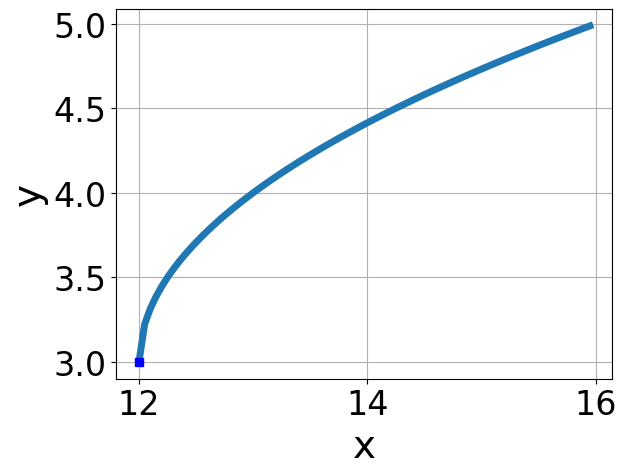
\includegraphics[width=0.5\textwidth]{../Figures/radicalGraphToEquationCopyC.png}
\end{center}
\begin{enumerate}[label=\Alph*.]
\item \( f(x) = \sqrt{x - 10} + 7 \)
\item \( f(x) = \sqrt{x + 10} + 7 \)
\item \( f(x) = - \sqrt{x + 10} + 7 \)
\item \( f(x) = - \sqrt{x - 10} + 7 \)
\item \( \text{None of the above} \)

\end{enumerate} }
\litem{
Solve the radical equation below. Then, choose the interval(s) that the solution(s) belongs to.\[ \sqrt{-54 x^2 - 18} - \sqrt{93 x} = 0 \]\begin{enumerate}[label=\Alph*.]
\item \( x_1 \in [-1.54, -1.37] \text{ and } x_2 \in [-1.96,-0.08] \)
\item \( x \in [-1.23,1.19] \)
\item \( x \in [-1.54,-1.37] \)
\item \( x_1 \in [1.43, 2.19] \text{ and } x_2 \in [0.01,0.73] \)
\item \( \text{All solutions lead to invalid or complex values in the equation.} \)

\end{enumerate} }
\litem{
What is the domain of the function below?\[ f(x) = \sqrt[7]{-9 x - 3} \]\begin{enumerate}[label=\Alph*.]
\item \( (-\infty, \infty) \)
\item \( \text{The domain is } (-\infty, a], \text{   where } a \in [-1.33, 2.67] \)
\item \( \text{The domain is } [a, \infty), \text{   where } a \in [-0.8, 0.9] \)
\item \( \text{The domain is } (-\infty, a], \text{   where } a \in [-7, -1] \)
\item \( \text{The domain is } [a, \infty), \text{   where } a \in [-4.7, -1.9] \)

\end{enumerate} }
\litem{
Solve the radical equation below. Then, choose the interval(s) that the solution(s) belongs to.\[ \sqrt{-7 x - 4} - \sqrt{-3 x - 6} = 0 \]\begin{enumerate}[label=\Alph*.]
\item \( x \in [0.29,1.38] \)
\item \( \text{All solutions lead to invalid or complex values in the equation.} \)
\item \( x_1 \in [-0.7, -0.55] \text{ and } x_2 \in [0.1,2.2] \)
\item \( x_1 \in [-2.24, -1.59] \text{ and } x_2 \in [-1.9,-0.3] \)
\item \( x \in [-3.06,-2.35] \)

\end{enumerate} }
\litem{
Solve the radical equation below. Then, choose the interval(s) that the solution(s) belongs to.\[ \sqrt{6 x - 8} - \sqrt{9 x - 9} = 0 \]\begin{enumerate}[label=\Alph*.]
\item \( x_1 \in [0.77, 1.72] \text{ and } x_2 \in [0.33,6.33] \)
\item \( \text{All solutions lead to invalid or complex values in the equation.} \)
\item \( x \in [-0.74,0.91] \)
\item \( x_1 \in [-0.74, 0.91] \text{ and } x_2 \in [0.33,6.33] \)
\item \( x \in [-6.57,-4.96] \)

\end{enumerate} }
\litem{
Solve the radical equation below. Then, choose the interval(s) that the solution(s) belongs to.\[ \sqrt{16 x^2 + 40} - \sqrt{56 x} = 0 \]\begin{enumerate}[label=\Alph*.]
\item \( x_1 \in [-5.9, -1.2] \text{ and } x_2 \in [-4,1] \)
\item \( \text{All solutions lead to invalid or complex values in the equation.} \)
\item \( x \in [-0.8,1.9] \)
\item \( x_1 \in [-0.8, 1.9] \text{ and } x_2 \in [0.5,5.5] \)
\item \( x \in [1.5,3.3] \)

\end{enumerate} }
\end{enumerate}

\end{document}